\section{Testing}
\label{testing}
\subsection{Setup}
To test our image processing- and mapping system I will be using a tripod with a built in bulls eye spirit level to ensure the image sensor is normal to the ground- and wall plane when capturing an image. 
\begin{figure}[H]
\centering
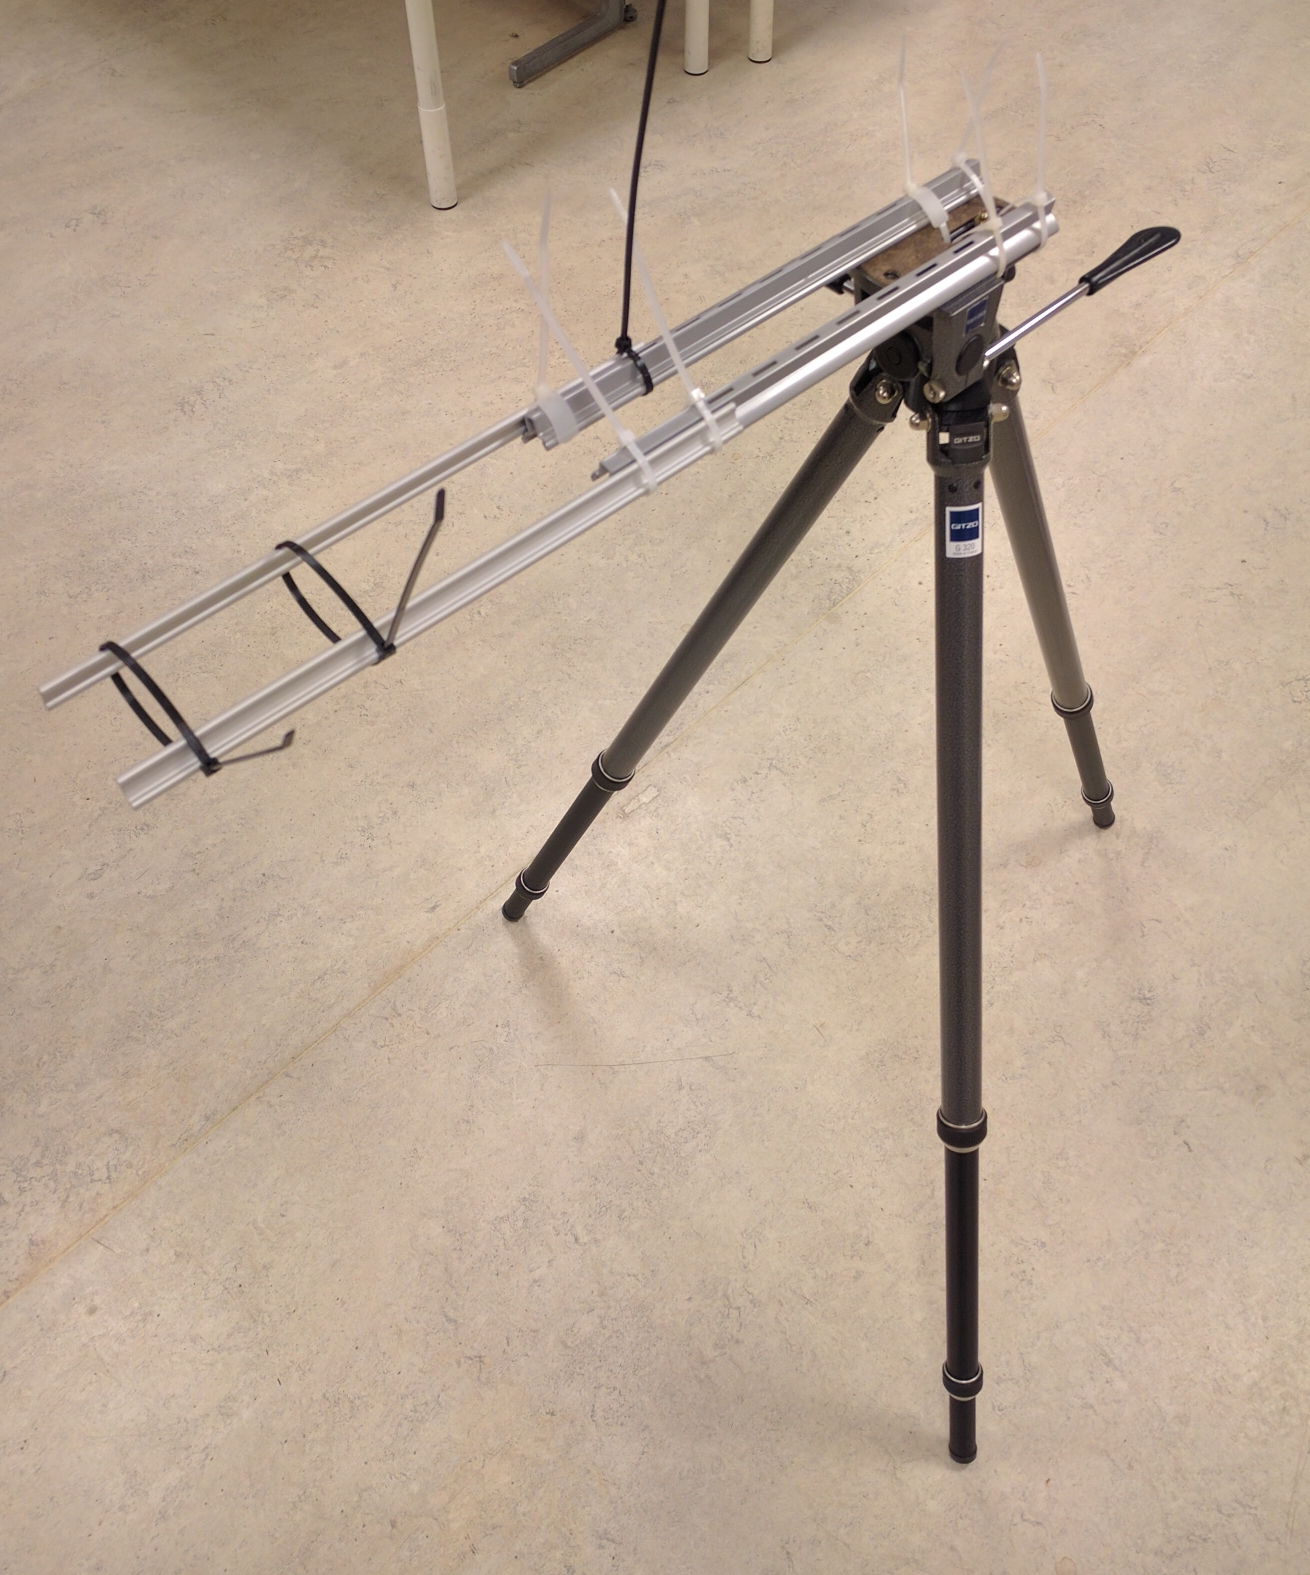
\includegraphics[width=0.9\textwidth]{fig/tripod}
  \caption{Tripod used for testing}
  \label{fig:tripod}
\end{figure}
\begin{figure}[H]
\centering
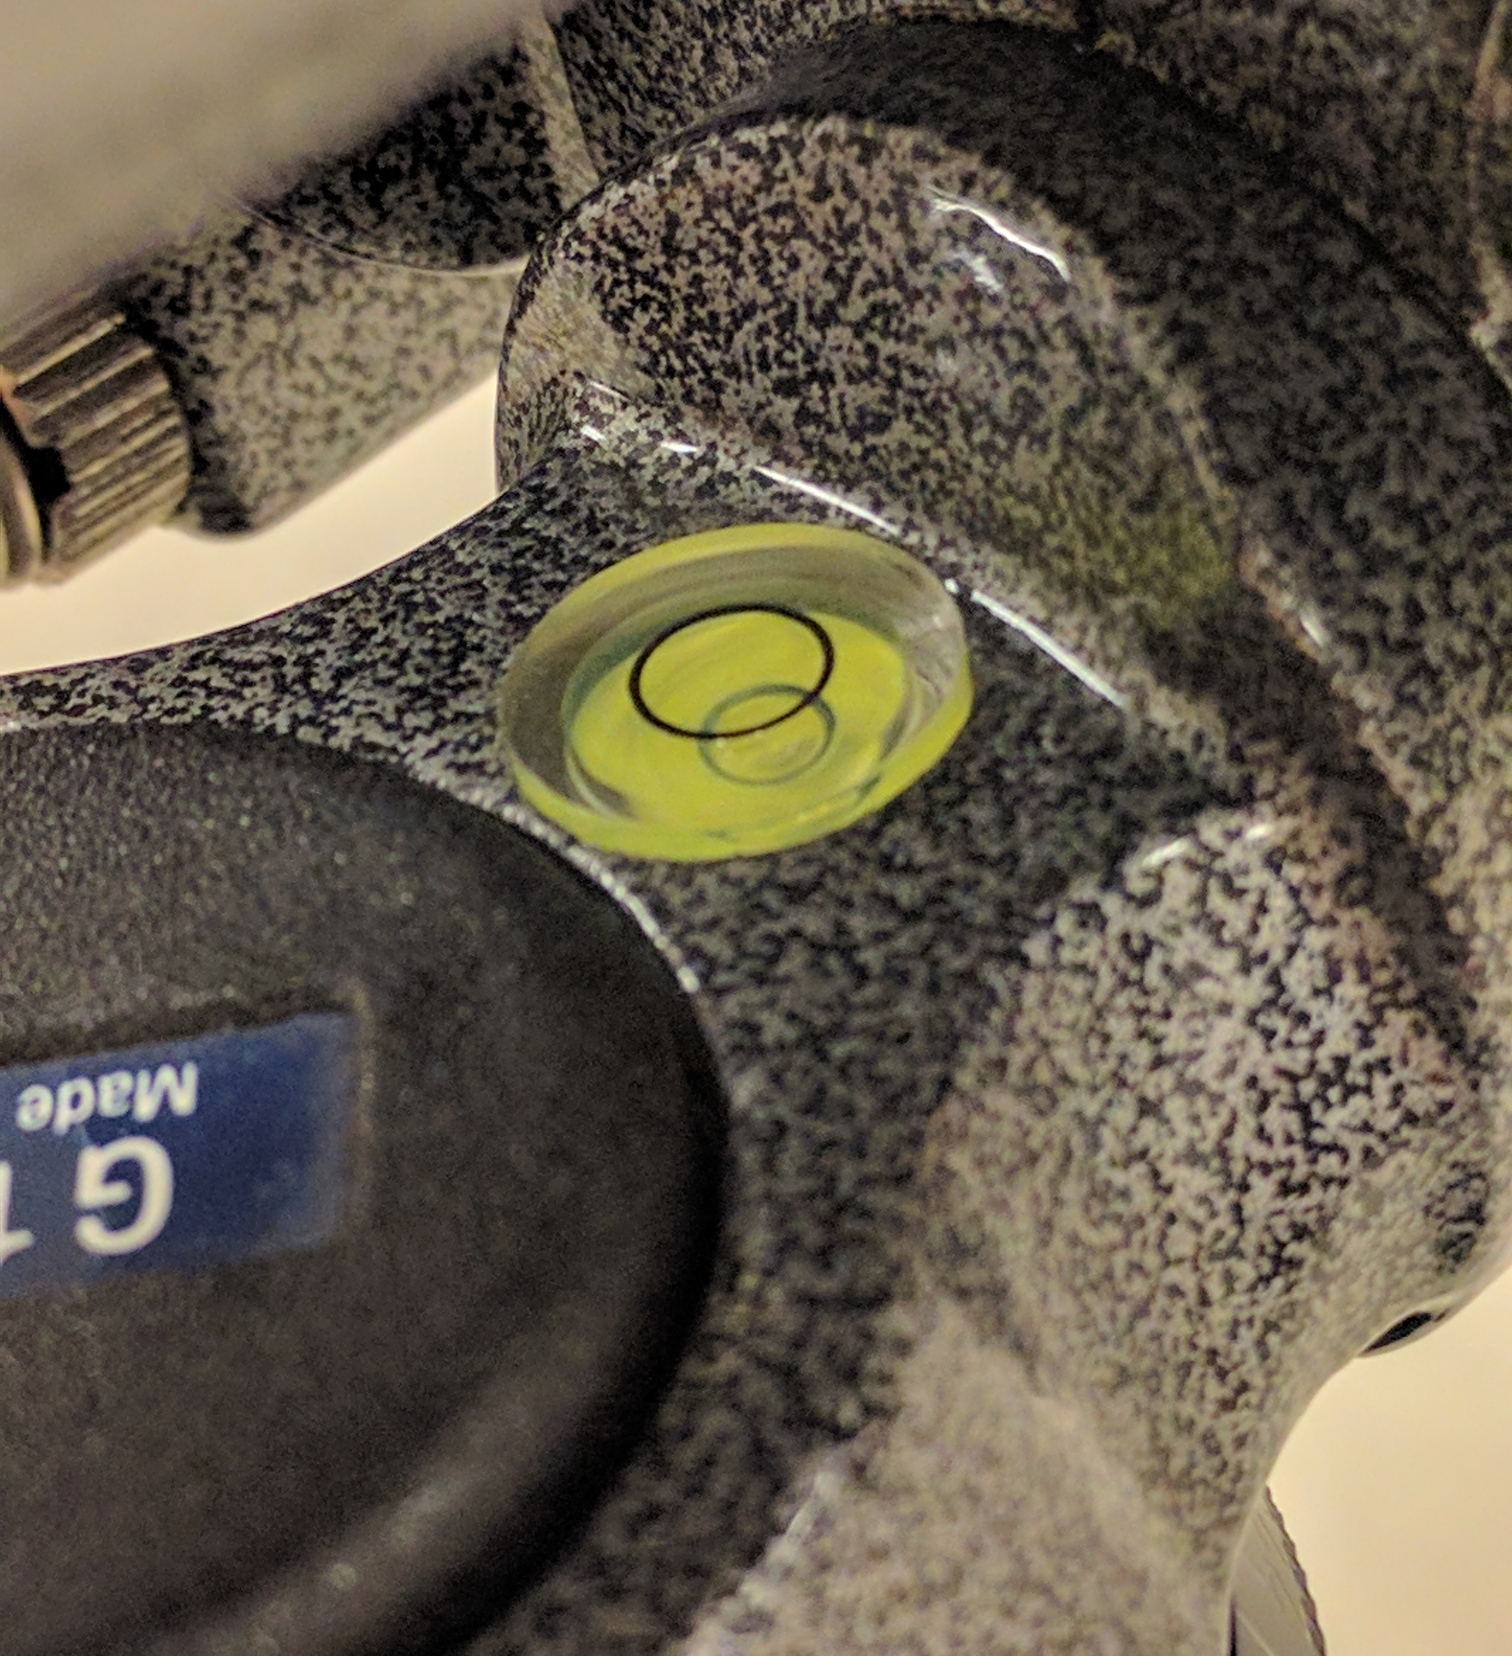
\includegraphics[width=0.9\textwidth]{fig/vater}
  \caption{Bulls eye spirit level on the tripod}
  \label{fig:vater}
\end{figure}
The tripod is equipped with configurable legs to adjust the height of the tripod. These will be used to adjust the height while keeping the spirit level in the center at each measured height. The height itself will be measured by a measuring tape from the optic normal to the ground. 
\begin{figure}[H]
\centering
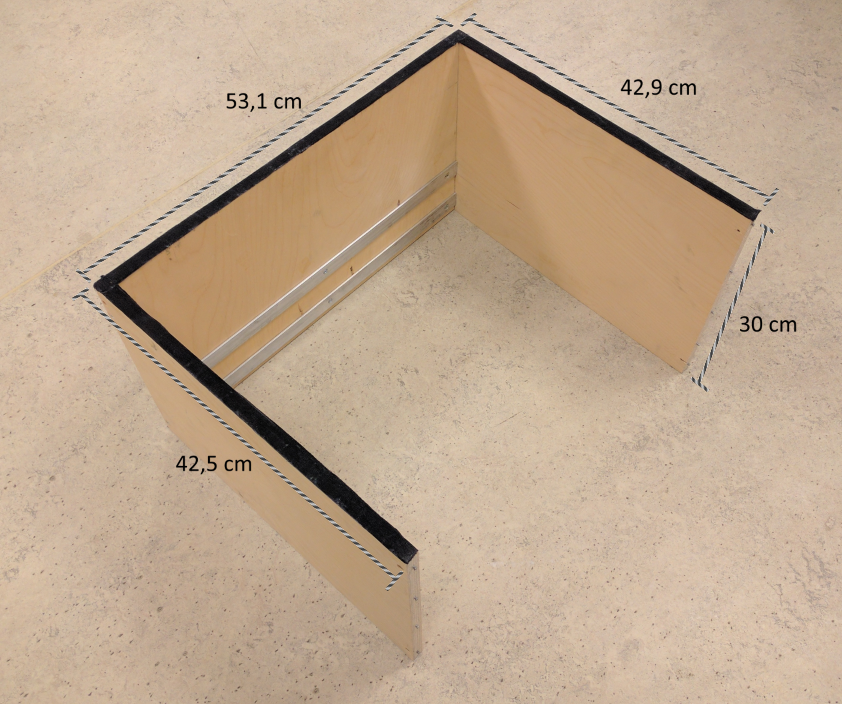
\includegraphics[width=0.9\textwidth]{fig/maze}
  \caption{Test maze}
  \label{fig:maze}
\end{figure}
We will be using a test maze with the real life lengths and heights described in Figure \ref{fig:maze}. This is the charging station for the Lego-robots and is designed to be a part of a bigger maze setup. This is a simplification of the environment the complete system will be designed to operate in, but will serve for testing purposes only.\\

The image sensor used will be a Sony Exmor IMX377:
\begin{figure}[H]
\centering
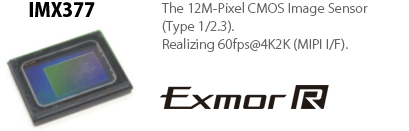
\includegraphics[width=0.9\textwidth]{fig/imx377}
  \caption{IMX377 Image sensor}
  \label{fig:sensor}
\end{figure}

\newpage



\subsection{Distortion moving away from the focal center}
\label{lens}
One of the ways to test the accuracy of the assumed theory is to see if by moving the object further away from the focal center of the image, the calculated lengths of the wall changes. We can test this by placing our test-wall at three different locations in the image, and calculate the wall lengths and compare them.\\

Figure \ref{ltest} shows the three different images (a) to (c), complete with edge detection. The values shown along the walls are the pixel value lengths of the edge segments detected in the image. During these tests, the image was scaled by a factor of $0.3$ in order to get complete edge detection along the walls for all the images using the same Canny parameters for all the images. The center of the image is marked with a green cross. I will be testing on the back wall, since this wall is the wall that is most consistently completely detected. The two edge lengths of the back wall will be averaged to one length for testing.\\

Calculating GSD:
\begin{align*}
S_W = 6,17 \quad \textbf{(Sensor width of camera [mm])}\\
F_R = 4,67 \quad \textbf{(Focal length of the camera [mm])}\\
H_p = 1,3 \quad \textbf{Height from image sensor to wall [m]}\\
W_I = 4000 \quad \textbf{Image width [pixels]}\\
H_I = 2994 \quad \textbf{Image height [pixels]}\\\\
GSD = S_W \times Height \times 100 / (F_R \times W_I) = 0,042938972 \quad [cm/pixel]
\end{align*}
If we look at the top horizontal wall in the image and use the calculated GSD above, we can determine the physical lengths of the top wall in the three pictures. They can be calculated as:
\begin{align*}
(a)\quad L_{top} = 1245\times 0,042938972 = 53,459\quad[cm]\\
(b)\quad L_{top} = 1251\times 0,042938972 = 53,716\quad[cm]\\
(c)\quad L_{top} = 1260\times 0,042938972 = 54,103\quad[cm]
\end{align*}
We can see that we experience a difference of $+0.644$ cm in length of the top wall when the maze is moved further away from the focal center. This is most likely because of lens distortion, and will be discussed further in the discussion section of this report. This equates to about $1,2\%$ difference with respect to the actual wall length.
\begin{figure}[H]
\begin{subfigure}{.5\textwidth}
  \centering
  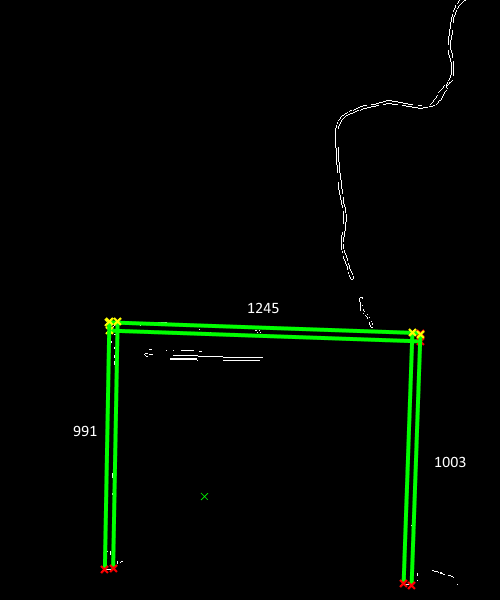
\includegraphics[width=.9\linewidth]{ltest1}
  \caption{}
\end{subfigure}
\begin{subfigure}{.5\textwidth}
  \centering
  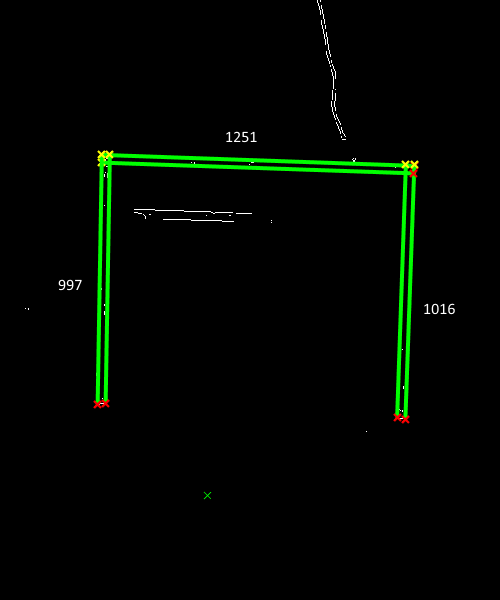
\includegraphics[width=.9\linewidth]{ltest2}
  \caption{}
\end{subfigure}
\begin{subfigure}{.5\textwidth}
  \centering
  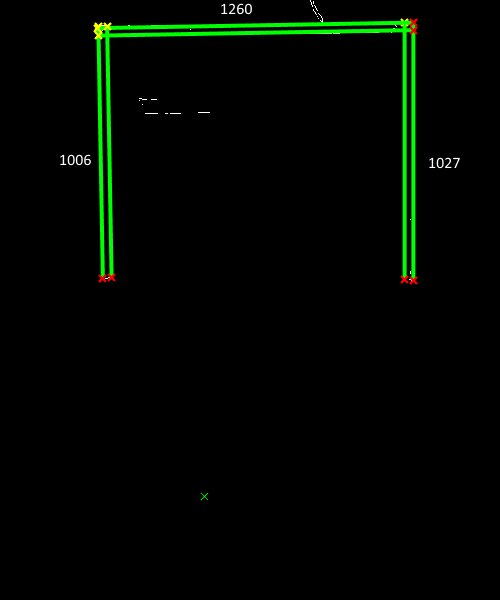
\includegraphics[width=.9\linewidth]{ltest3}
  \caption{}
\end{subfigure}
\caption{Test of length in terms of distance from focal center.}
\label{ltest}
\end{figure}

\subsection{Accuracy of varying height}
\label{varyingheight}
There are several key insights in testing the edge detection algorithm and Hough transform in varying height environments. What we want to test is if the computed real life length of the walls remain constant as we vary the height of the image sensor. The setup limits us to only being able to check for the lengths of the walls, as we cannot guarantee and control the same xy-position of the image sensor when varying height.
\begin{table}[H]
\centering
\begin{tabular}{l|l|l|l|}
\cline{2-4}
                              & Height above ground & Height above wall & GSD\\ \hline
\multicolumn{1}{|l|}{Image 1} & 159,5 cm            & 129,5 cm          & 0,042773822\\ \hline
\multicolumn{1}{|l|}{Image 2} & 145,6 cm            & 115,6 cm          & 0,038182655\\ \hline
\multicolumn{1}{|l|}{Image 3} & 114,2 cm            & 84,2 cm           & 0,027811242\\ \hline
\multicolumn{1}{|l|}{Image 4} & 101,0 cm            & 71,0 cm           & 0,023451285\\ \hline
\end{tabular}
\caption{Height information}
\label{height}
\end{table}
Like explained in the previous test, the back wall will be used for comparison since this is the wall with the most consistent complete detection. Table \ref{height} displays the different heights and GSD for each of the images used in this test. Keep in mind, one important factor that affects this test is that the Canny algorithm variables will need to be tuned for each height to suppress the non-important edges in the image. This is a potential source of error since the tuning variables are crucial for good edge detection, and do not remain constant during the test.


\begin{figure}[h]
\begin{subfigure}{.5\textwidth}
  \centering
  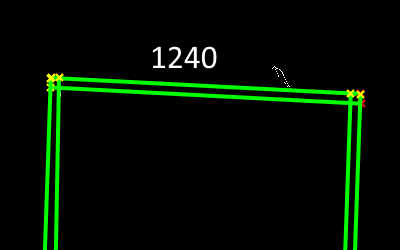
\includegraphics[width=.9\linewidth]{ltest11}
  \caption{Image 1}
\end{subfigure}
\begin{subfigure}{.5\textwidth}
  \centering
  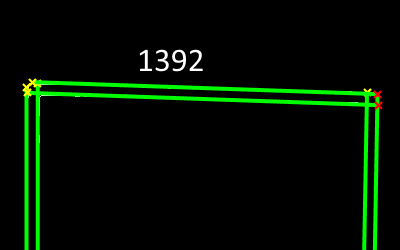
\includegraphics[width=.9\linewidth]{ltest22}
  \caption{Image 2}
\end{subfigure}
\begin{subfigure}{.5\textwidth}
  \centering
  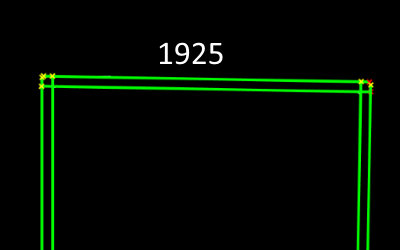
\includegraphics[width=.9\linewidth]{ltest33}
  \caption{Image 3}
\end{subfigure}
\begin{subfigure}{.5\textwidth}
  \centering
  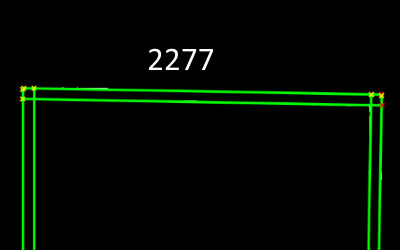
\includegraphics[width=.9\linewidth]{ltest44}
  \caption{Image 4}
\end{subfigure}
\caption{Test of length in terms of varying height}
\label{htest}
\end{figure}
Computing the real-life length of the back wall with the respective GSD for each image:
\begin{align*}
\textbf{Length Image 1} = 1240*0,042773822 = 53,0395\quad[cm]\\
\textbf{Length Image 2} = 1392*0,038182655 = 53,1503\quad[cm]\\
\textbf{Length Image 3} = 1925*0,027811242 = 53,5366\quad[cm]\\
\textbf{Length Image 4} = 2277*0,023451285 = 53,3985\quad[cm]
\end{align*}
It is important to note that what we are looking for in this test is the change of computed wall length, not the accuracy of the actual computation compared to the real life wall. Looking at the results, the computed length of the back wall is different in each computation. With measurements ranging from $53.0395$ [cm] to $53.5366$ [cm] we have a maximum difference of the measurements which is less that one percent of the total length of the wall:
\begin{align*}
\frac{53,5366-53,0395}{53.1}\quad= 0,0093 = 0,93\%
\end{align*}

\subsection{Sensitivity to error in height measurement}
It might prove a useful insight to measure how sensitive our system is to errors in the height measurement of the image sensor. This is partly to see how accurate our position sensor in the complete system needs to be to obtain the demanded accuracy. One way to test for sensitivity is to have an accurate mapping of an image compared to the real life test maze, and change the height variable in the calculation of the GSD while seeing how much of an effect a change of height measurement will have on the computed lengths.\\

We can use the measurement of Image 2 in the last section and change the measured height by 1\% and see how much the computed length of the wall changes. We have:
\begin{align*}
GSD_{Image 2} = \frac{Sw\times H_p\times 100}{Fr\times Iw} = \frac{6,17\times1,156\times100}{4,67\times4000} = 0,038182655\\
\textbf{Length Image 2} = 1392*0,038182655 = 53,1503\quad[cm]
\end{align*}
If we change the height variable $H_p$ by 1\% from $115.6$ [cm] to $1.01\times 115.6 = 116.756$ [cm] we have:
\begin{align*}
GSD_{Image 2} = \frac{Sw\times H_p\times 100}{Fr\times Iw} = \frac{6,17\times1,16756\times100}{4,67\times4000} = 0,038182655\\
\textbf{Length Image 2} = 1392*0,038564482 = 53,6817\quad[cm]
\end{align*}
We can calculate the percentage of change in the computed length of the wall as:
\begin{align*}
\frac{0,038564482}{0,038182655} = 1,01
\end{align*}
This is almost exactly $+1\%$ increase in GSD from introducing an error of $+1\%$ to the height measurement. In real life units this means that the GSD is linearly dependent on the measurement of height. This can be also seen from the equation for GSD. With the current setup, a small change in height of $+1$ [cm] changed the computed length of the back wall by about $+0.5$ [cm]. 

\subsection{Actual accuracy of GSD method with accurate height}
\label{actualgsd}
Using Image 4 in the previous section, it is possible to check the accuracy of the computation relative to the actual real life maze. We have the following information about Image 4:
\begin{align*}
H_p = 0,71 \quad [m]\\
GSD_{Image 4} = 0,023451285
\end{align*}
Using the implementation from Section \ref{implementation} we with the above variables we will get the following Hough transform plot and real-life plot:
\begin{figure}[H]
\centering
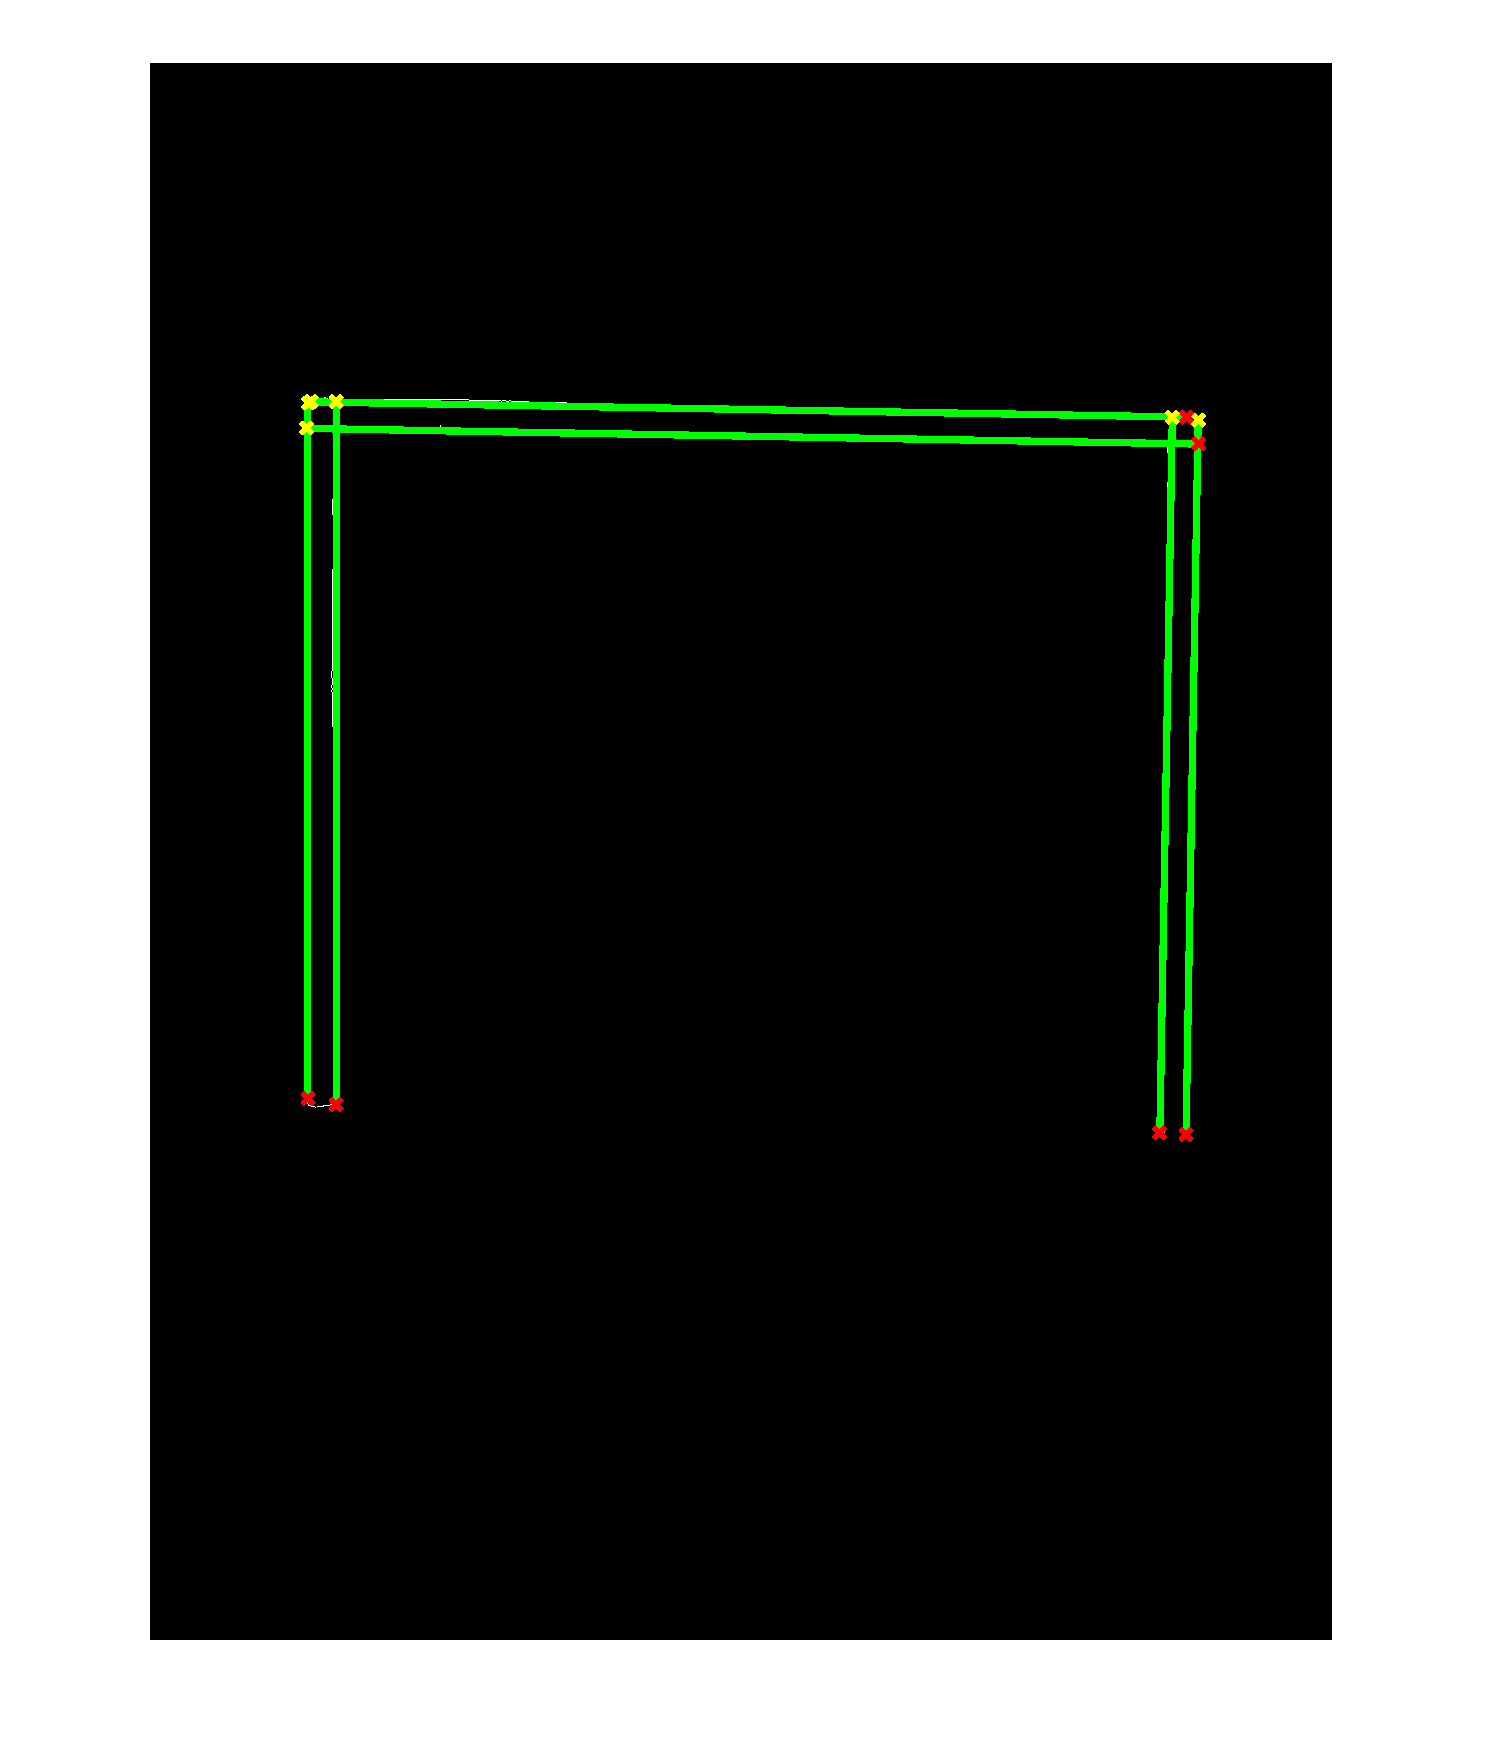
\includegraphics[width=0.5\textwidth]{fig/GSDmethod}
  \caption{Hough transform plot}
  \label{fig:GSDmethod1}
\end{figure}
\begin{figure}[H]
\centering
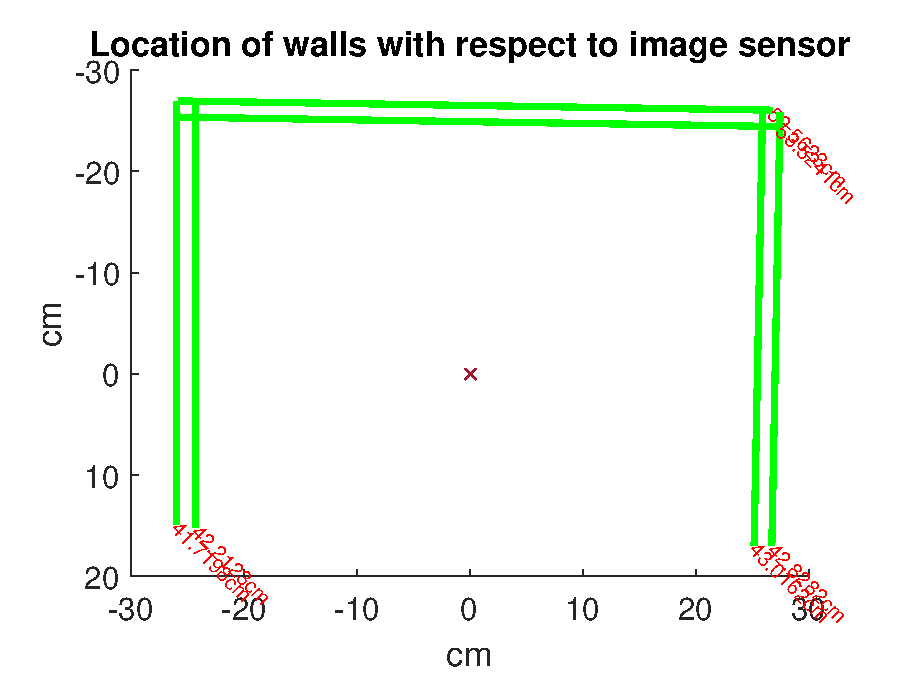
\includegraphics[width=0.9\textwidth]{fig/GSDmethod2}
  \caption{Real-life plot}
  \label{fig:GSDmethod2}
\end{figure}

From Figure \ref{fig:GSDmethod2} we get the following values:
\begin{align*}
\textbf{Length Left Wall} = 41,7198\quad[cm] \quad and \quad42,2123\quad[cm]\\
\textbf{Length Back Wall} = 52,5623\quad[cm] \quad and \quad53,5241\quad[cm]\\
\textbf{Length Right Wall} = 43,0162\quad[cm] \quad and \quad42,8282\quad[cm]
\end{align*}
We have the actual maze characteristics:
\begin{align*}
\textbf{Length Left Wall} = 42,5\quad[cm]\\
\textbf{Length Back Wall} = 53,1\quad[cm]\\
\textbf{Length Right Wall} = 42,9\quad[cm]
\end{align*}
As one can see from Figure \ref{fig:GSDmethod2} we get two length values for the walls. One for each edge on the top of the wall. The values are more often that not different, meaning that we get two different estimates for the wall lengths. By looking closer at the corners of the mapped maze it is possible to detect why this is the case:
\begin{figure}[H]
\centering
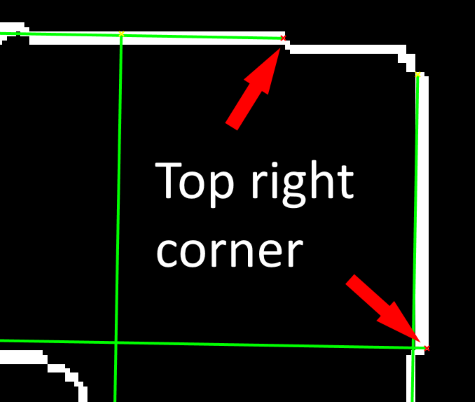
\includegraphics[width=0.6\textwidth]{fig/error}
  \caption{Top right corner of Hough plot}
  \label{fig:error}
\end{figure}
From Figure \ref{fig:error} the end points on the top edge of the top wall and the bottom edge of the top wall does not end at the same place. The edges are detected and marked, since there is no gap in the white part of the figure, but the Hough transform fails to extend to the end of the wall, and ends prematurely. This will be discussed further in the sources of error section. On the other hand, looking at the actual mapping, the algorithm does not map the last part of the top edge of the top wall, which means that it actually does give a correct length measurement, but for a shortened part of the top wall:
\begin{figure}[H]
\centering
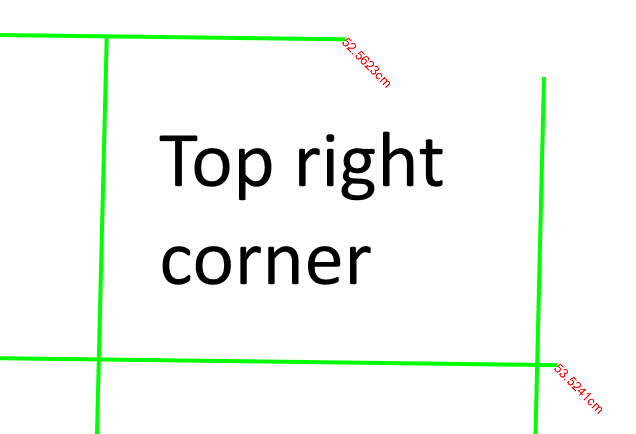
\includegraphics[width=0.7\textwidth]{fig/error2}
  \caption{Top right corner of mapping}
  \label{fig:error2}
\end{figure}
By choosing to select the value of the two lengths calculated per wall section which is the closest to the real life length we can compare them:
\begin{align*}
\Delta\textbf{Length Left Wall} = 42,2123-42,5 = -0,2887\quad [cm]\\
\Delta\textbf{Length Back Wall} = 53,5241-53,1 = 0,4241\quad [cm]\\
\Delta\textbf{Length Right Wall} = 43,0162-42,9 = 0,1162\quad [cm]
\end{align*}

This means that when the height is measured correctly, the accuracy of our algorithm and implementation is within $\pm 0,5$ [cm] margin of the actual real life lengths of the wall in this test. This will be discussed further and compared to the Lego-robots in the discussion section later.\\

Although this result is very positive, we must realize this is an idealized test where the parameters have been tuned manually and by trial-and-error. There is no way of knowing the system will be this accurate before we have a complete maze where we mount the image sensor on a UAV. The conditions might be different, and therefore the result will be different also. But on the other hand, this proves the legitimacy of the approach, and indicated that the implementation presented in this project will be beneficial for the overall project goal of mapping a maze.
















